\chapter{High Level}
\section{Overview}
High level part is responsible for the detection and recovery of Kidnap, which need the information from Kalman Filter and MCA\_ROS\_Bridge. The pose information can be obtained from EKF which merges the result from Kalman Filter in MCA and the output from Kinect. Besides, the data from odometry and laser scanner can be acquired through MCA. With the help of \texttt{spinner()} in ROS, the subscription of the topics from other groups and the publishment of our topics to other groups can be achieved in parallel . The structure of the whole software system is showed in Figure \ref{System}
\begin{figure}[ht]
\centering
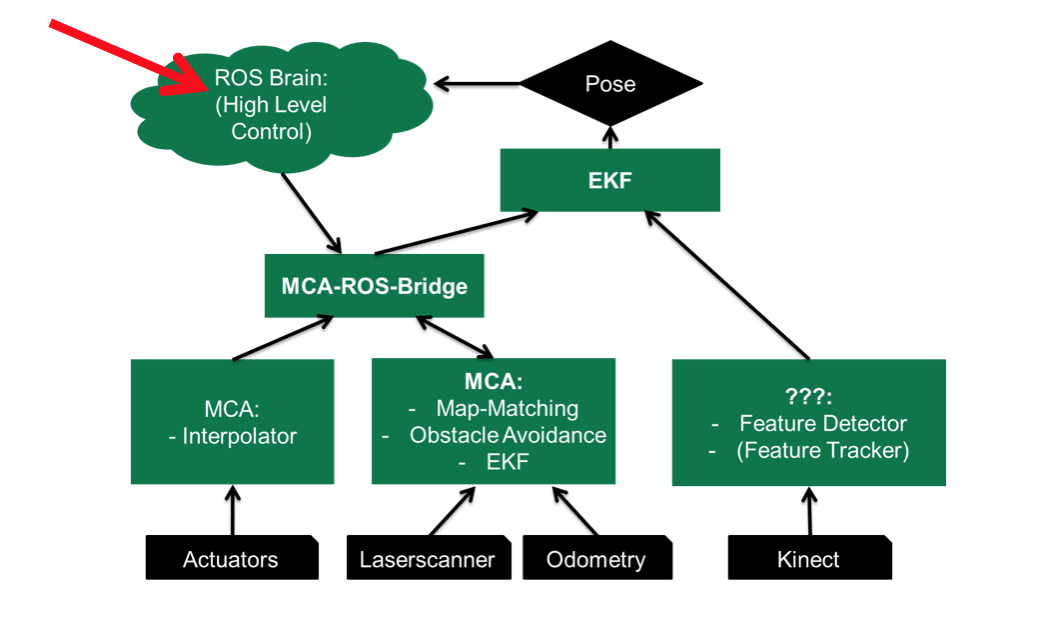
\includegraphics[width=0.4\textwidth]{graphics/system.png}
\caption{The structure of the whole software system}
\label{System}
\centering
\end{figure}

\section{Implementation}
\subsection{Detection}
Kidnap\_Detection was the first step that we used to solve kidnap problem. In this section, three criteria were taken into account to detect kidnap situation, namely timestamp of odometry, unexpected marker and hoch covariance. First of all, robot would regularly compare the current time with the timestamp of last message on topic \texttt{/robot/lauron/odom}. The difference between these two timestamps means that the robot has received no data from odometry for a while, which is most likely because of kidnap situation. Secondly, the robot subscribed the topic \texttt{/vision/unexpected\_marker}. When the robot receives an unexpected marker, it will be detected as kidnapped. Unexpected marker only occurs in such situation that the pose in robot’s mind is different from the real pose. When robot gets an unexpected marker, the covariance information on the topic \texttt{/kalman/fused\_pose} will be stored as the threshold for the third criterion. Kidnap situation happens normally with the hoch covariance of pose. With the saved covariance, robot can detect kidnap situation when the covariance is large enough. Because random variables are independent, there exists only the variance of random variables in the covariance matrix. We didn’t consider the variance of Yaw, because these data from MCA were with large fluctuation thus not reliable through the observation. This is also the reason why we saved the covariance matrix from Kalman Filter on receiving the unexpected marker rather than the timestamps. The detection will be done if some new information arrives. When no new data come, the Kidnap\_detection is done every 2 seconds.

In the beginning, we searched for some detection methods through papers, then finally decided to use the “strong change of covariance” as our kidnap detection criterion, which can be represented in a second-order derivative. However, we could only obtain a little data from Kalman Filter about kidnap situation, so it was difficult to define “strong” with the real data. Therefore, we directly used the covariance matrix. There are still some other methods to achieve the detection such as using the Map-Matching confidence rate, particle filter.

\subsection{Recovery}
\subsubsection{Concept}
Kidnap\_Recovery is the second step to solve the kidnap problem. After determining whether kidnapped, Pfosten will go over the whole room to search for QR code or other features, through which  Pfosten can relocalize and set a new pose up. The basic concept to achieve this goal is a maze-solving algorithm, which keeps the robot moving along the left side of obstacles. This algorithm will be described in details in the next capital. The robot should go over every corner without colliding with obstacles, so it needs some sensors such as laser scanner and odometry. Finally, after seeing the marker, the exploration comes to end and Pfosten calculates the transformation between Frame  \texttt{/local\_map} and \texttt{/global\_map} instead of setting a pose. Concerning about safety, various driving speeds were defined in the exploration for the robot in different zones, which depend on the distances to the obstacles in the environment. Figure \ref{Zone} details this idea. The closer the robot is to the obstacle, the slower it is. When the distance between the laser scanner and the obstacle becomes less than 0.11m, the robot should stop. When distance is less than 0.3m, the robot should move slowly.

\begin{figure}[ht]
\centering
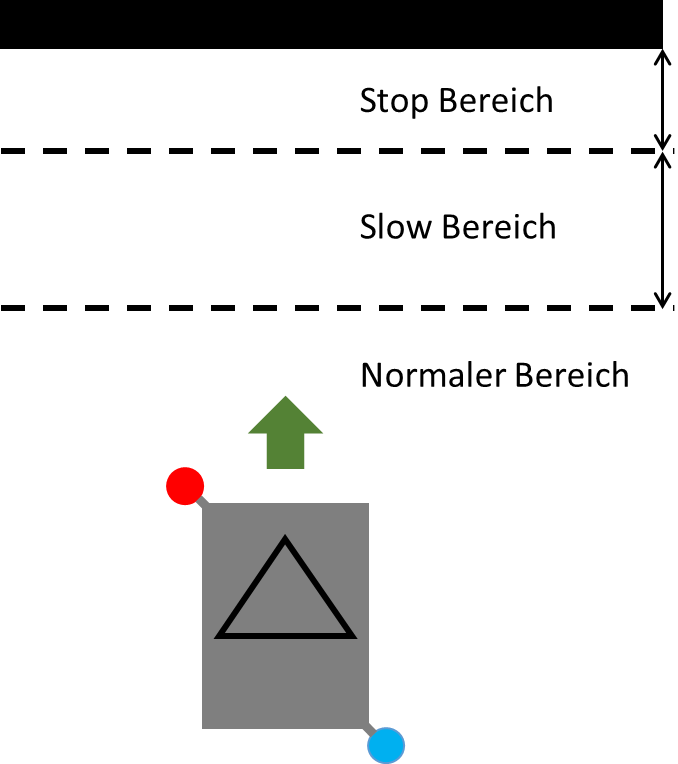
\includegraphics[width=0.4\textwidth]{graphics/Zone.png}
\caption{Definition of various speeds depending on obstacles}
\label{Zone}
\centering
\end{figure}

\subsubsection{Initial Actions}
Firstly, Pfosten stops after noticing Kidnap and then rotates itself to observe the environment, as shown in Figure \ref{sensor}. The distance between the obstacle and the robot, read from laser scanner, will be stored in the robot. After 360 degrees, the minimal distance and the angle will be filtered as \texttt {best\_angle}, which is shown in Figure \ref{best}. The robot rotates continually to \texttt {best\_angle} and goes forward to this obstacle. When the robot is near the obstacle, it will adjust itself until it is parallel to the edge of the obstacle, which is detailed in Figure \ref{parallel}.

\begin{figure}[ht]
\centering
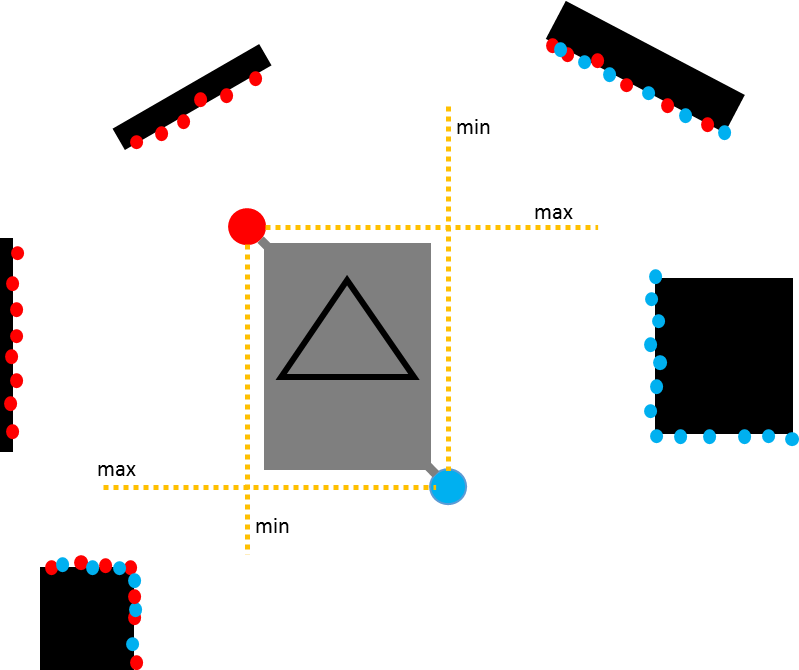
\includegraphics[width=0.4\textwidth]{graphics/sensoren.png}
\caption{Observation of the environment}
\label{sensor}
\centering
\end{figure}

\begin{figure}[ht]
\centering
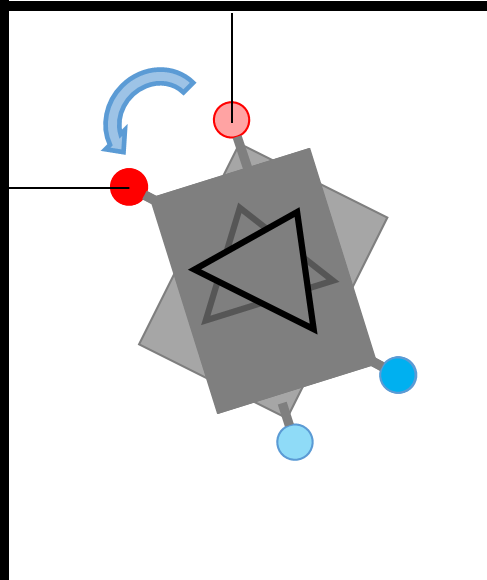
\includegraphics[width=0.4\textwidth]{graphics/find_best_angle.png}
\caption{Find best\_angle}
\label{best}
\centering
\end{figure}

\begin{figure}[ht]
\centering
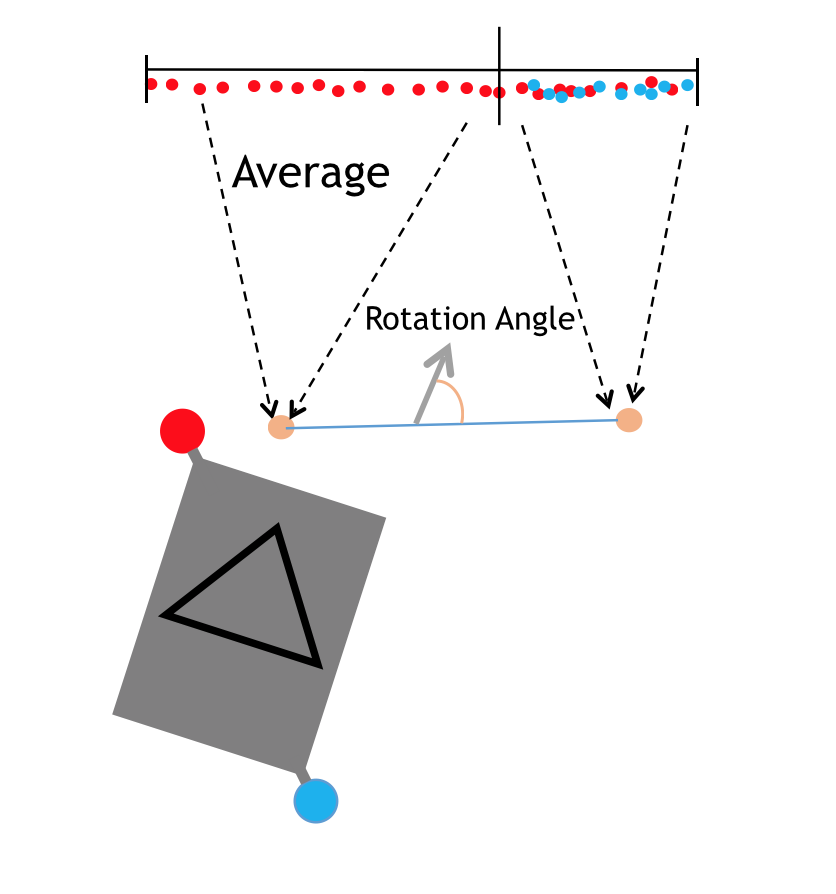
\includegraphics[width=0.4\textwidth]{graphics/front_parallel.png}
\caption{Rotate to fit the obstacle}
\label{parallel}
\centering
\end{figure}

\subsubsection{Exploration}

\section{Problems and Difficulties}
\subsection{Calibration}
\subsection{Floor Level}
\subsection{Uneven Surface}
\subsection{Transparent Window}